\chapter{构建垫片三维模型}\label{chap:dianpian}

{\bfseries 学习目标}
\begin{itemize}
\item 学习利用layer命令管理图层和设置图线
\item 学习利用xline命令绘制辅助线
\item 学习利用arrayploay建立环形阵列
\item 学习利用cylinder命令进行圆柱体的三维建模
\item 学习利用3darray建立三维物体环形阵列
\item 掌握平面图形分析的基本方法
\end{itemize}

{\bfseries 任务要求}
\begin{itemize}
\item 根据图\ref{fig:tiaoyafadianpian}所示的零件图,用旋转法建立调压阀垫片零件的三维模型
\item 根据图\ref{fig:tiaoyafadianpian}所示的零件图,用拉伸法建立调压阀垫片零件的三维模型
\item 根据图\ref{fig:tiaoyafadianpian}所示的零件图,用实体建模法建立调压阀垫片零件的三维模型
\end{itemize}

\noindent
\begin{figure}[htbp]
\centering
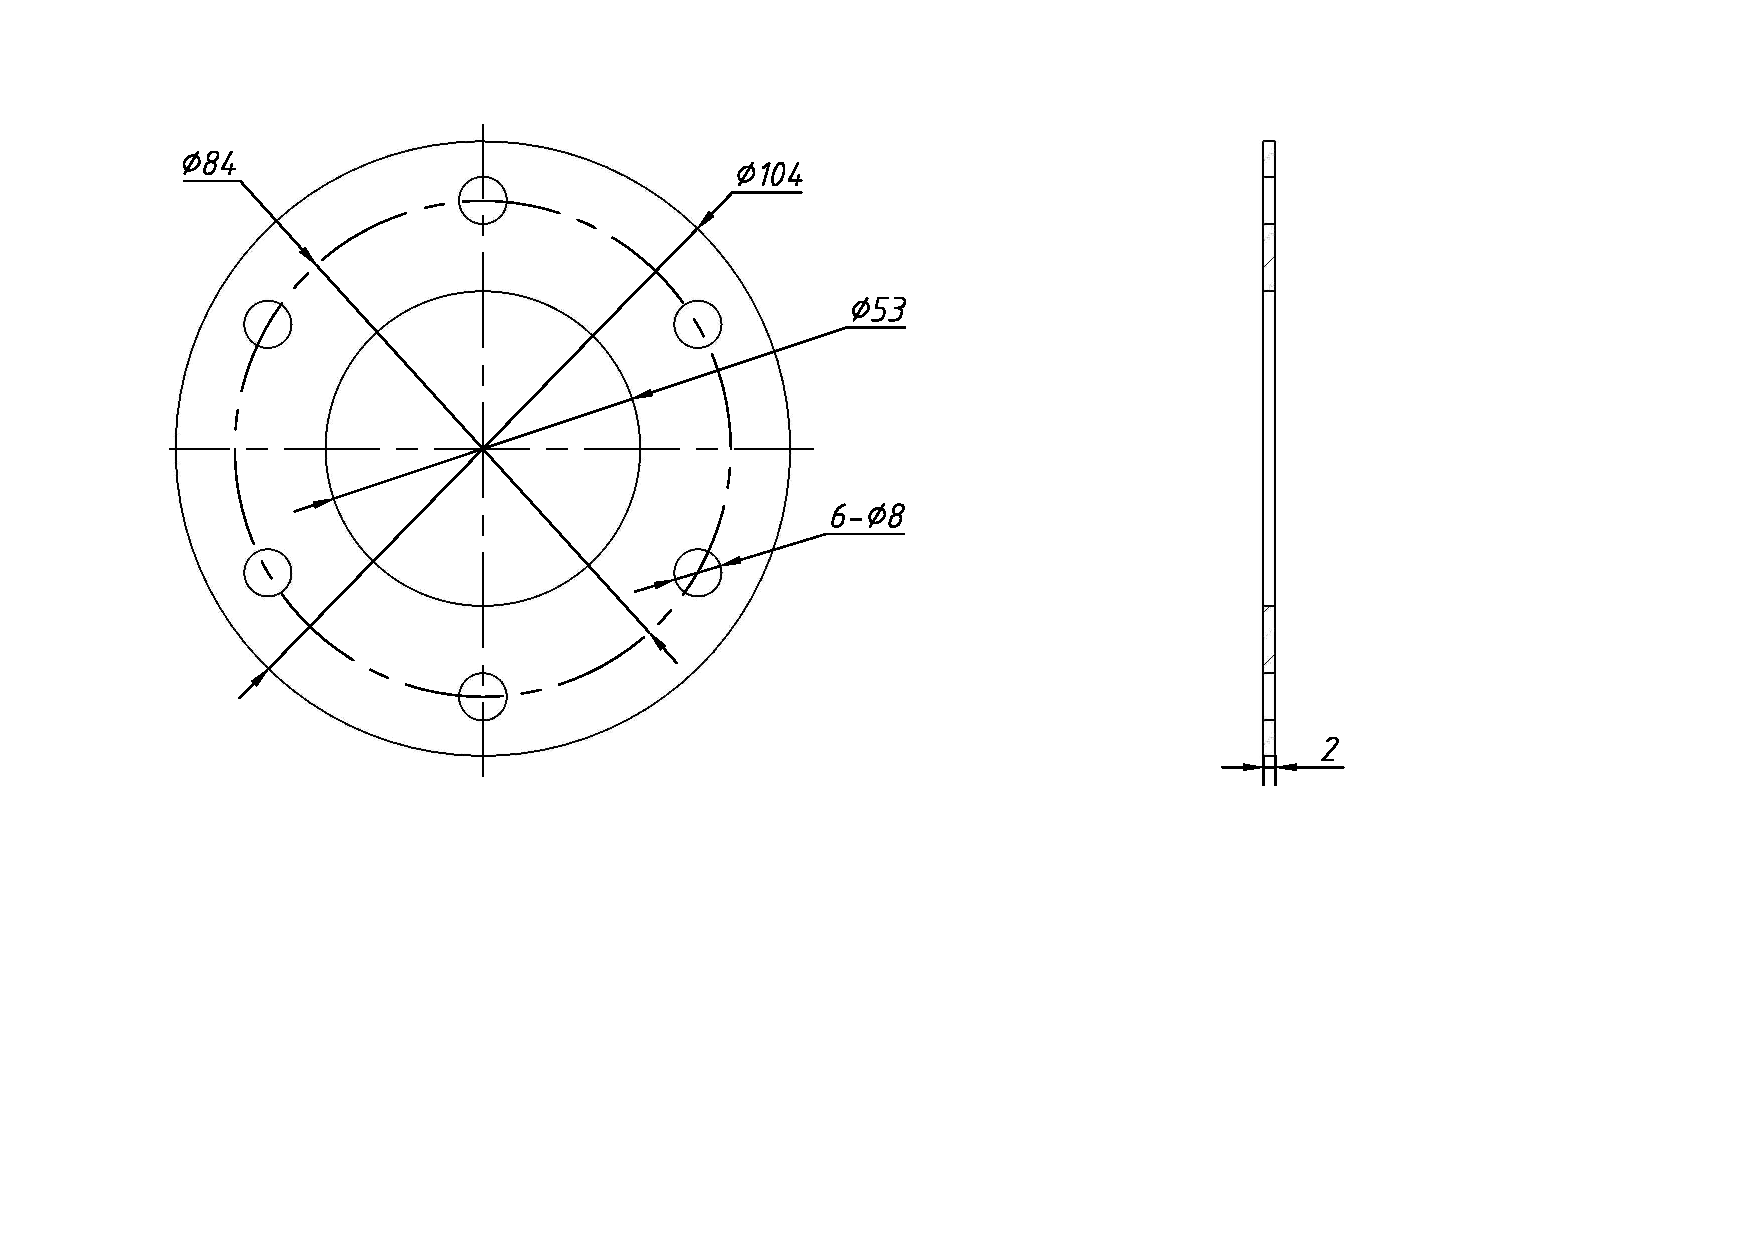
\includegraphics[scale=0.6]{tiaoyafadianpian.pdf}
\caption{垫片零件图}\label{fig:tiaoyafadianpian}
\end{figure}
\clearpage
平面图形分析是制图和三维建模工作中非常重要且很关键的步骤,是准确绘制图样和构建构模型的基础。平面图形分析的目的是分析和了解平面图形中各图形要素之间的相互位置关系,图形之间的依赖关系。图样中的各种尺寸是用于确定图样中图形对象的形状和位置。平面图分析是否准确、是否透彻,直接决定着绘图过程的正确性,也决定着能不能绘制图样和构建模型。

平面图形分析主要是进行平面图形的尺寸分析和平面图形要素的性质分析\footnote{平面图形要素性质分析也称为线段分析} 两个方面的内容。

\subsection{尺寸分析}
平面图形尺寸分析的目的是确定图形元素的尺寸基准、定形尺寸和定位尺寸。尺寸基准、定形尺寸和定位尺寸是平面图形尺寸分析的三大要素。

\begin{figure}[htbp]
\centering
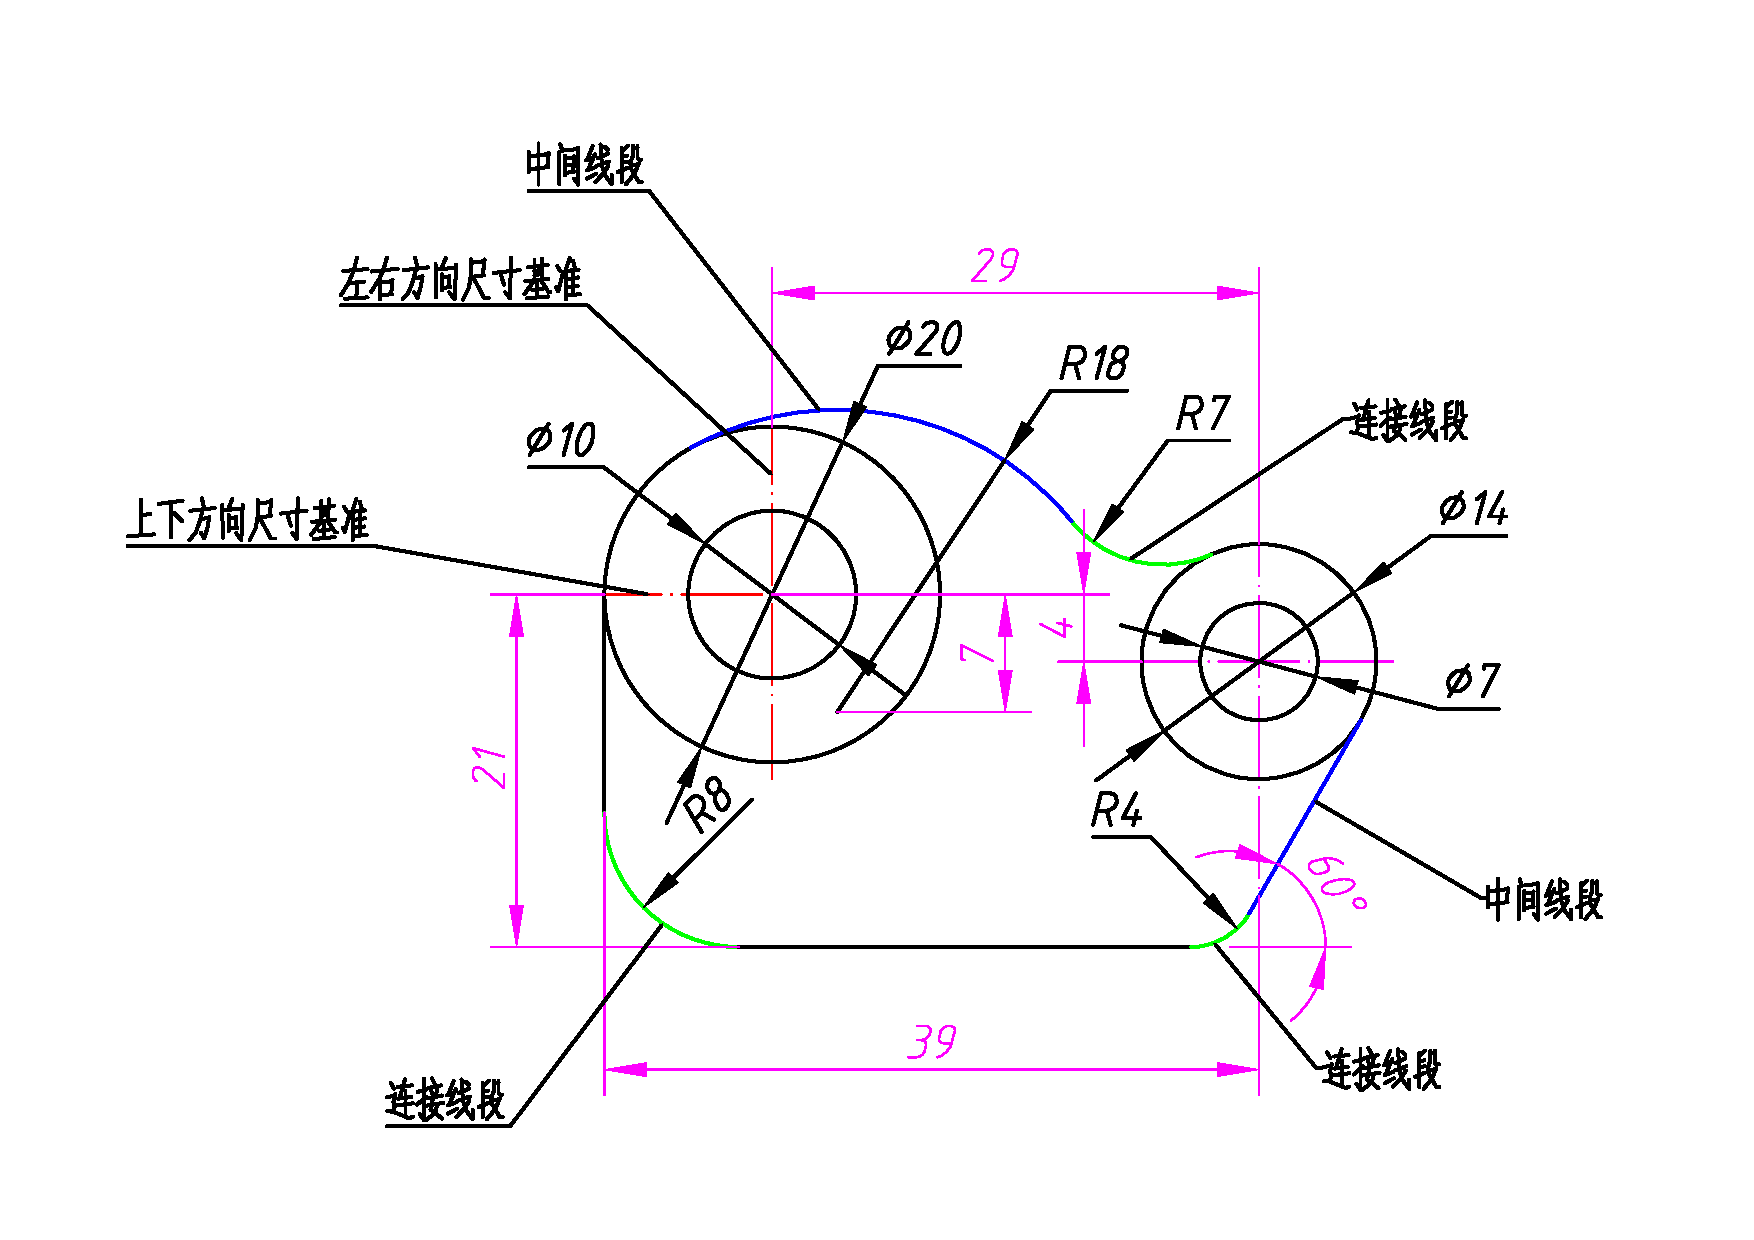
\includegraphics[scale=0.35]{biaozu.pdf}
\caption{平面图形的尺寸和线段分析} \label{fig:biaozu}
\end{figure}

\subsubsection{尺寸基准} 

尺寸基准是绘制和标注尺寸的起点,通常有水平和垂直两个方向的尺寸基准。实际工程图样中常采用图形的对称中心线,较大圆的中心线或主要轮廓线作为尺寸基准线。图\ref{fig:biaozu}所示图形主要是以长度为99mm的轮廓线和$\phi 20$圆的中心线作为垂直方向和水平方向的尺寸基准。

\subsubsection{定形尺寸} 

定形尺寸是确定平面图形中各种线段形状和大小的尺寸,如直线的长度、圆和圆弧的直径或半径、角度的大小等。图\ref{fig:biaozu6}中的$\phi 10$、$\phi 20$、 $\phi 14$、 $R8$、$R18$、$R7$等尺寸均为图\ref{fig:biaozu}的定形尺寸。

\begin{figure}[htbp]
\centering
\begin{floatrow}
\ffigbox{\caption{定形尺寸}\label{fig:biaozu6}}{
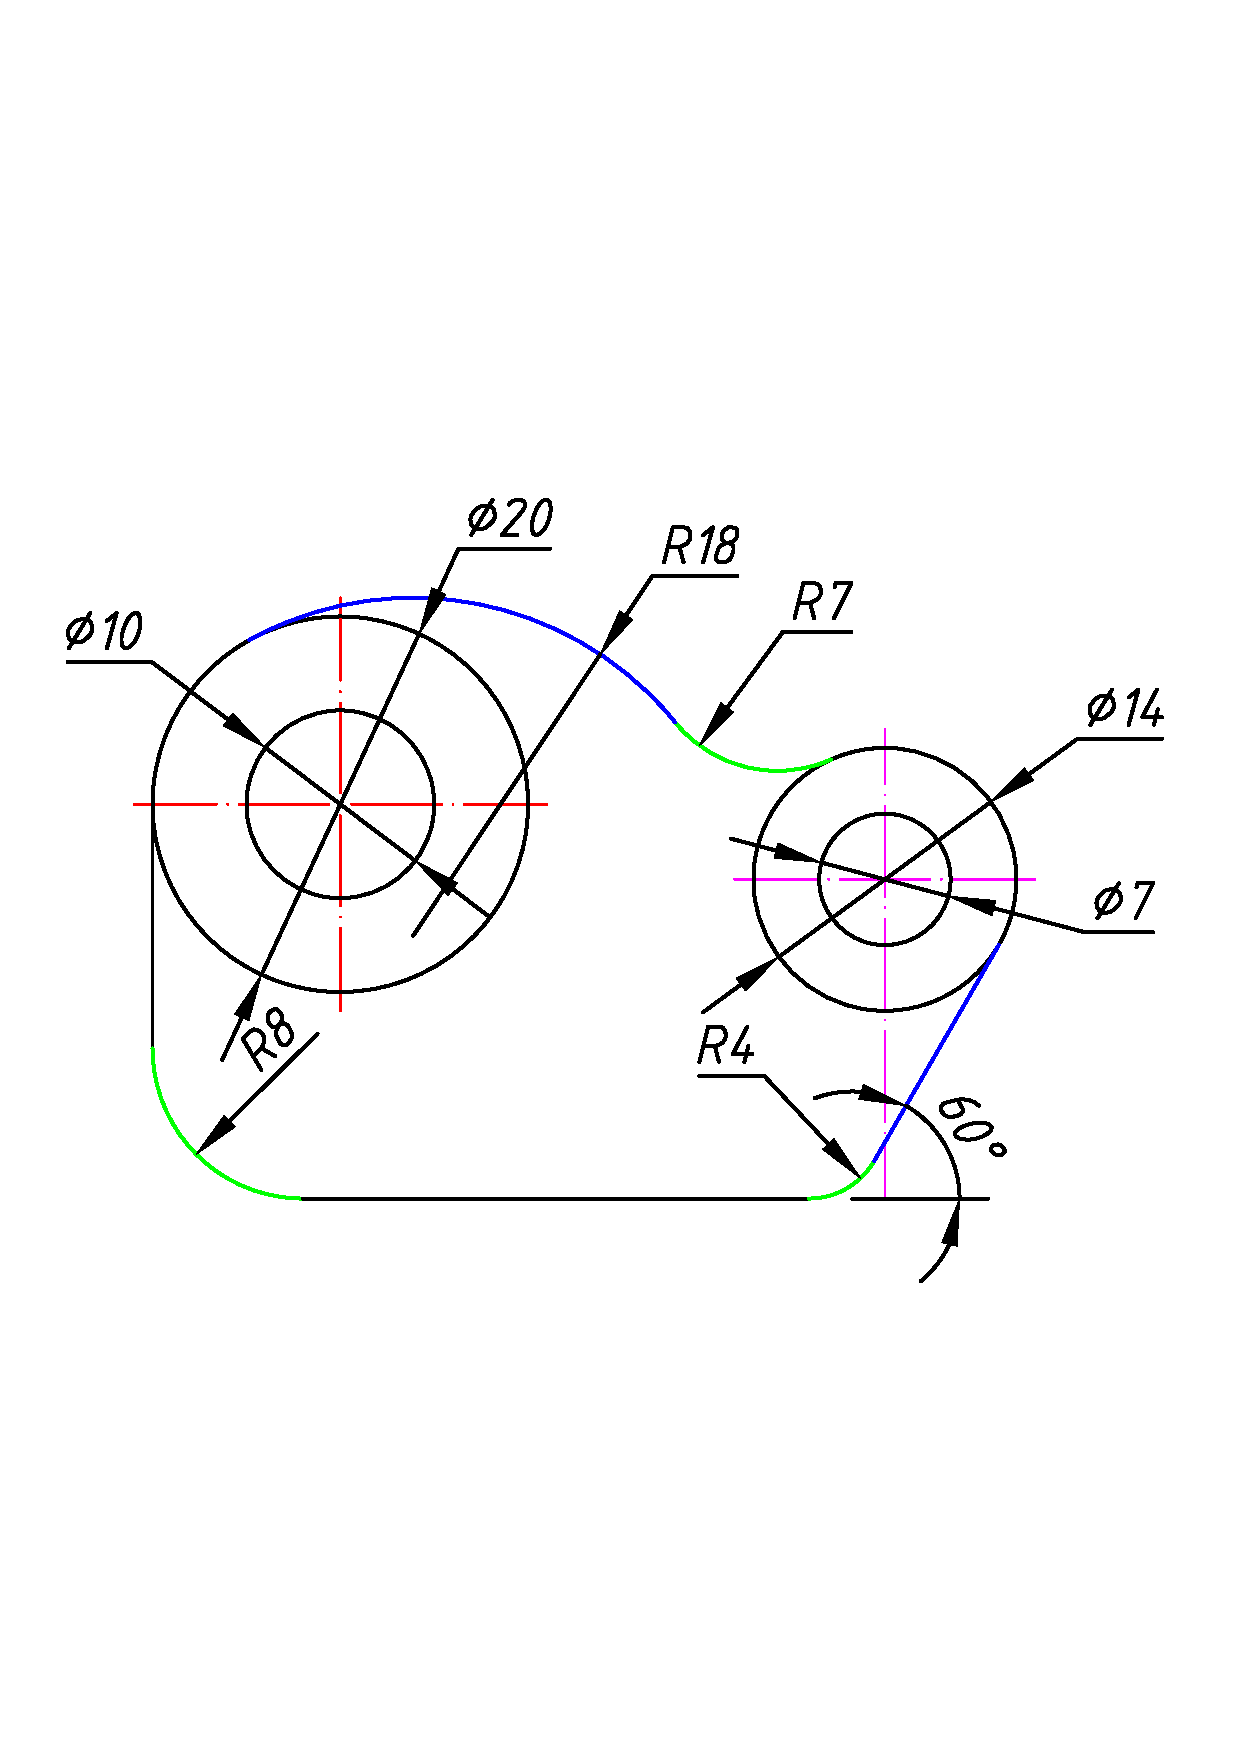
\includegraphics[scale=0.25]{biaozu6.pdf}
}
\ffigbox{\caption{定位尺寸}\label{fig:biaozu5}}{
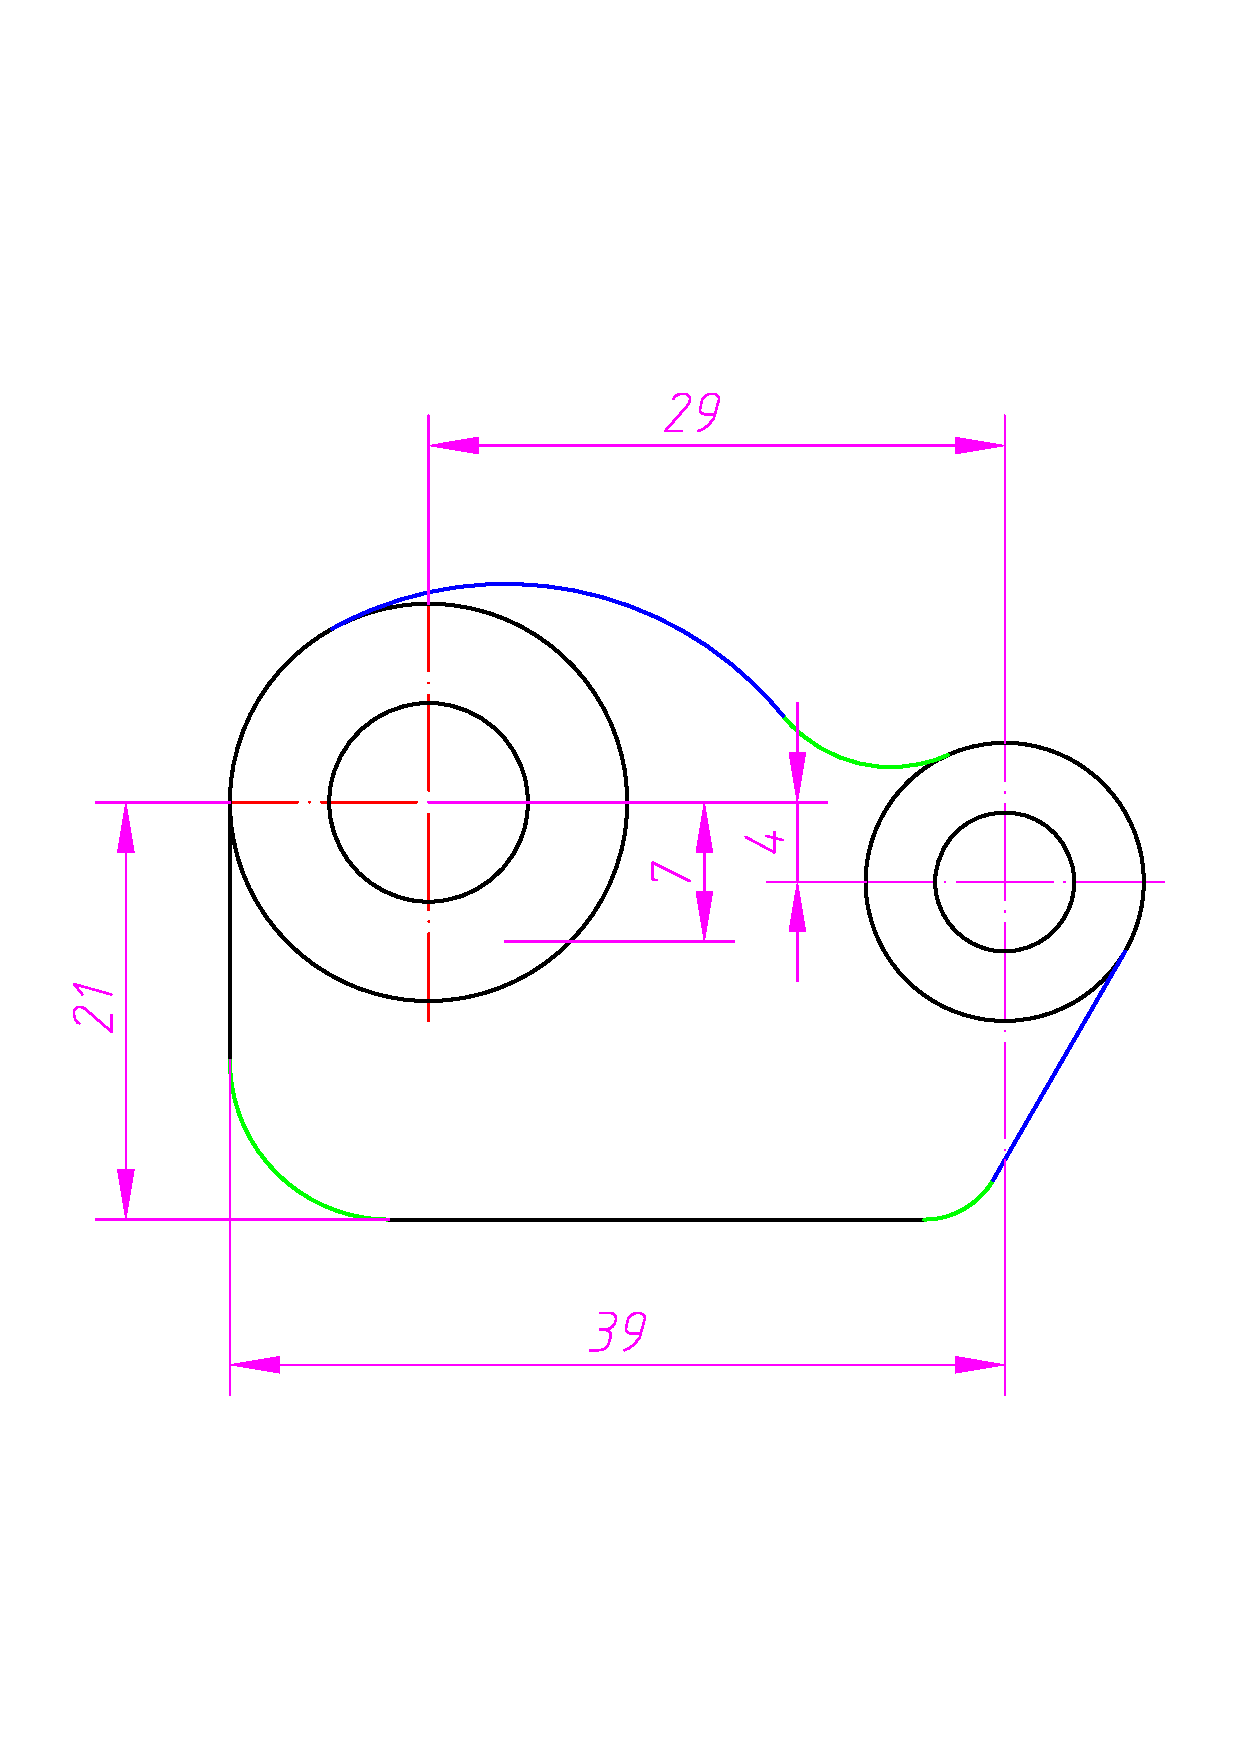
\includegraphics[scale=0.2]{biaozu5.pdf}
}
\end{floatrow}
\end{figure}

\subsubsection{定位尺寸} 

定位尺寸是确定平面图形中各线段之间相对位置的尺寸,图\ref{fig:biaozu5}中标出的尺寸均为图\ref{fig:biaozu}的定位尺寸,其中4和29用于确定$\phi 14$圆的圆心位置。

图\ref{fig:tiaoyafadianpian})中$\phi 104$圆的对称中心线是主视图的尺寸基准,$\phi 53,\phi 104,6-\phi 8$是定形尺寸,$\phi 104$圆的圆心和$\phi 84$为定位尺寸。

\endinput
\subsection{平面图形元素性质的分析}
平面图形中各线段(直线或圆弧)的定位尺寸的数量将直接影响绘图先后顺序,因此可将线段分为以下三类。

\subsubsection{已知线段}
已知线段是有足够的定位尺寸和定形尺寸,不需要利用与其它线段的连接关系即可直接画出的直线或圆弧。图\ref{fig:biaozu2}所示的即为图\ref{fig:biaozu}的已知线段。

\subsubsection{中间线段} 

中间线段是缺少一个定位尺寸,需要通过与它相邻某一边的图线的连接关系,才能够作出的直线或圆弧。图\ref{fig:biaozu3}是在图\ref{fig:biaozu2}的基础上绘制出所有的中间线段。
\subsubsection{连接线段} 

连接线段是缺少两个定位尺寸,需要通过与它相邻两边图形的相切关系,才能够作出的直线或圆弧。图\ref{fig:biaozu4}是在图\ref{fig:biaozu3}的基础上进一步添加所有的连接线段。

\begin{figure}[htbp]
\centering
\subfloat[已知线段]{\label{fig:biaozu2}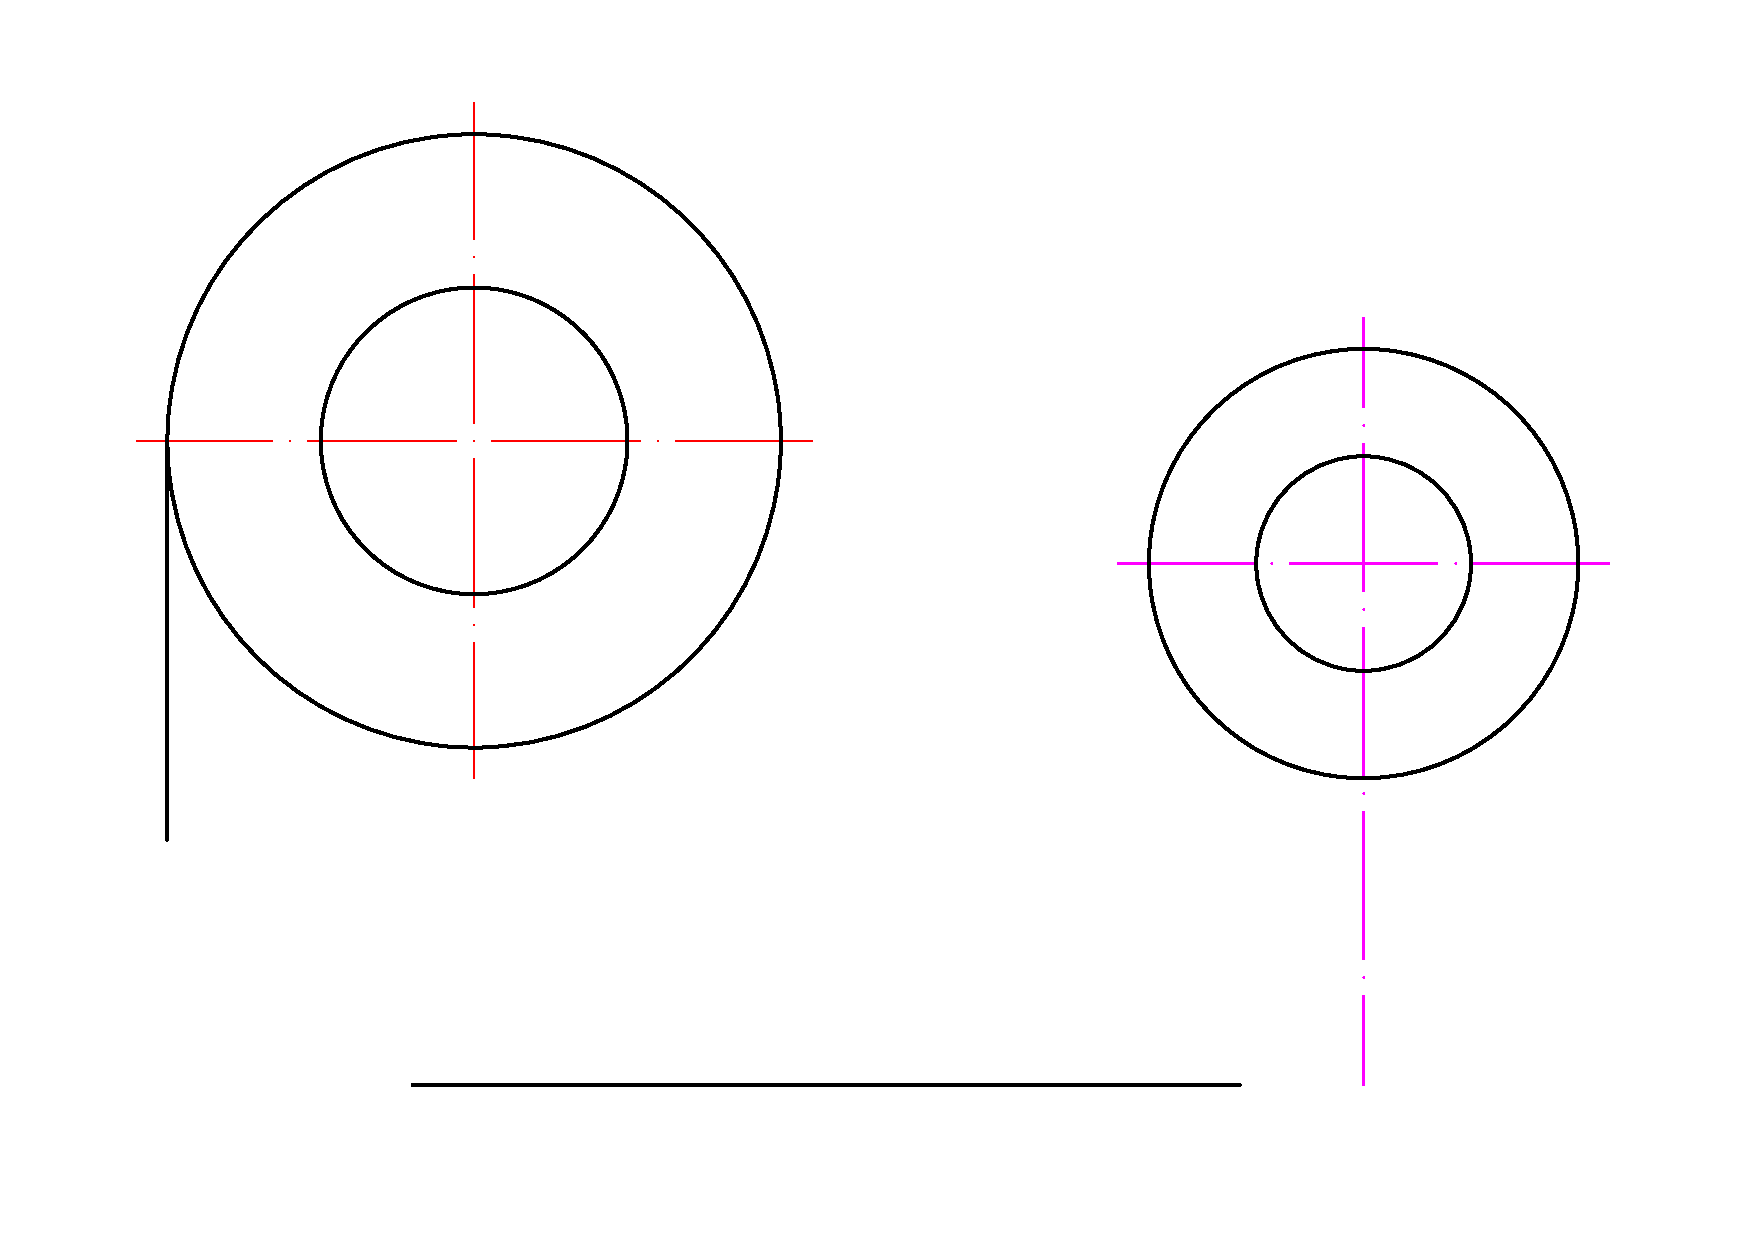
\includegraphics[scale=0.15]{biaozu2.pdf}}\hspace{20pt}
\subfloat[中间线段]{\label{fig:biaozu3}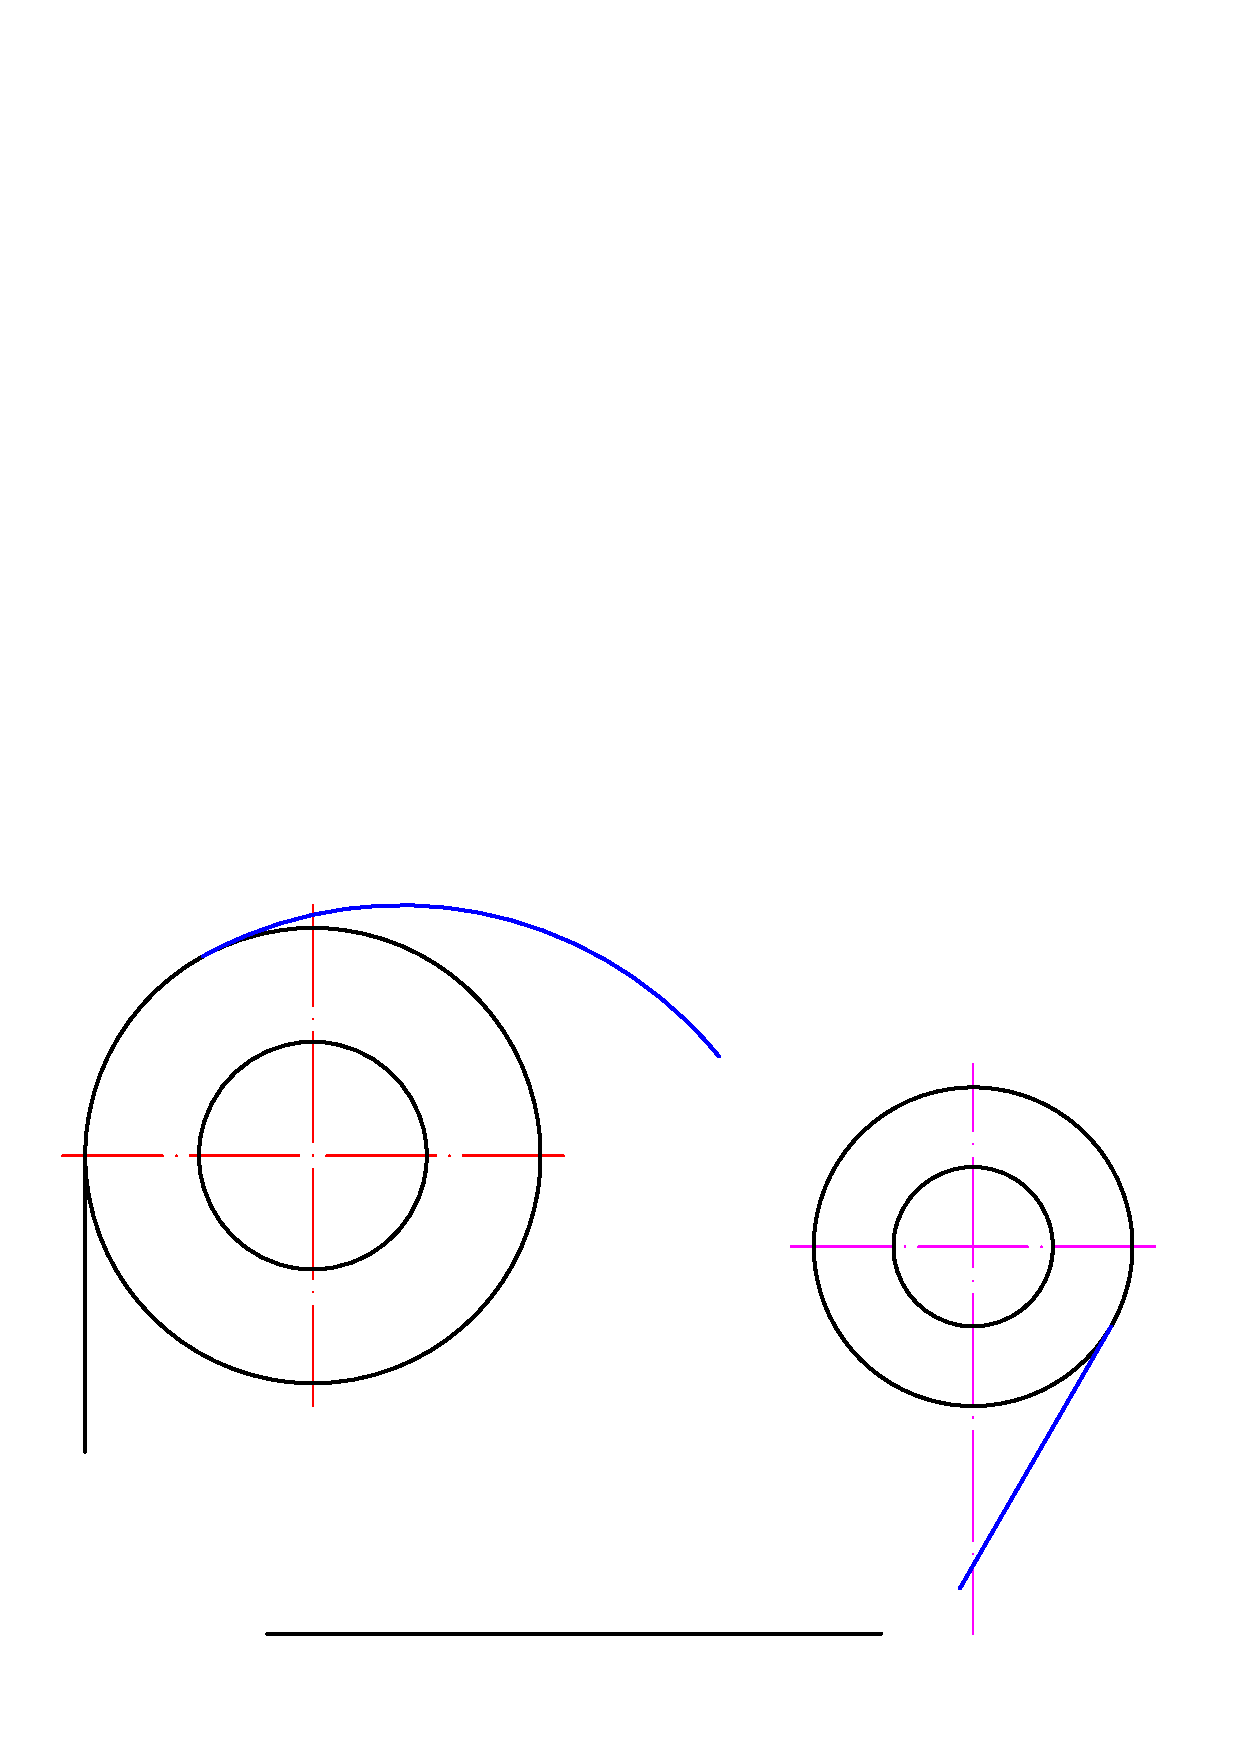
\includegraphics[scale=0.2]{biaozu3.pdf}}\hspace{20pt}
\subfloat[连接线段]{\label{fig:biaozu4}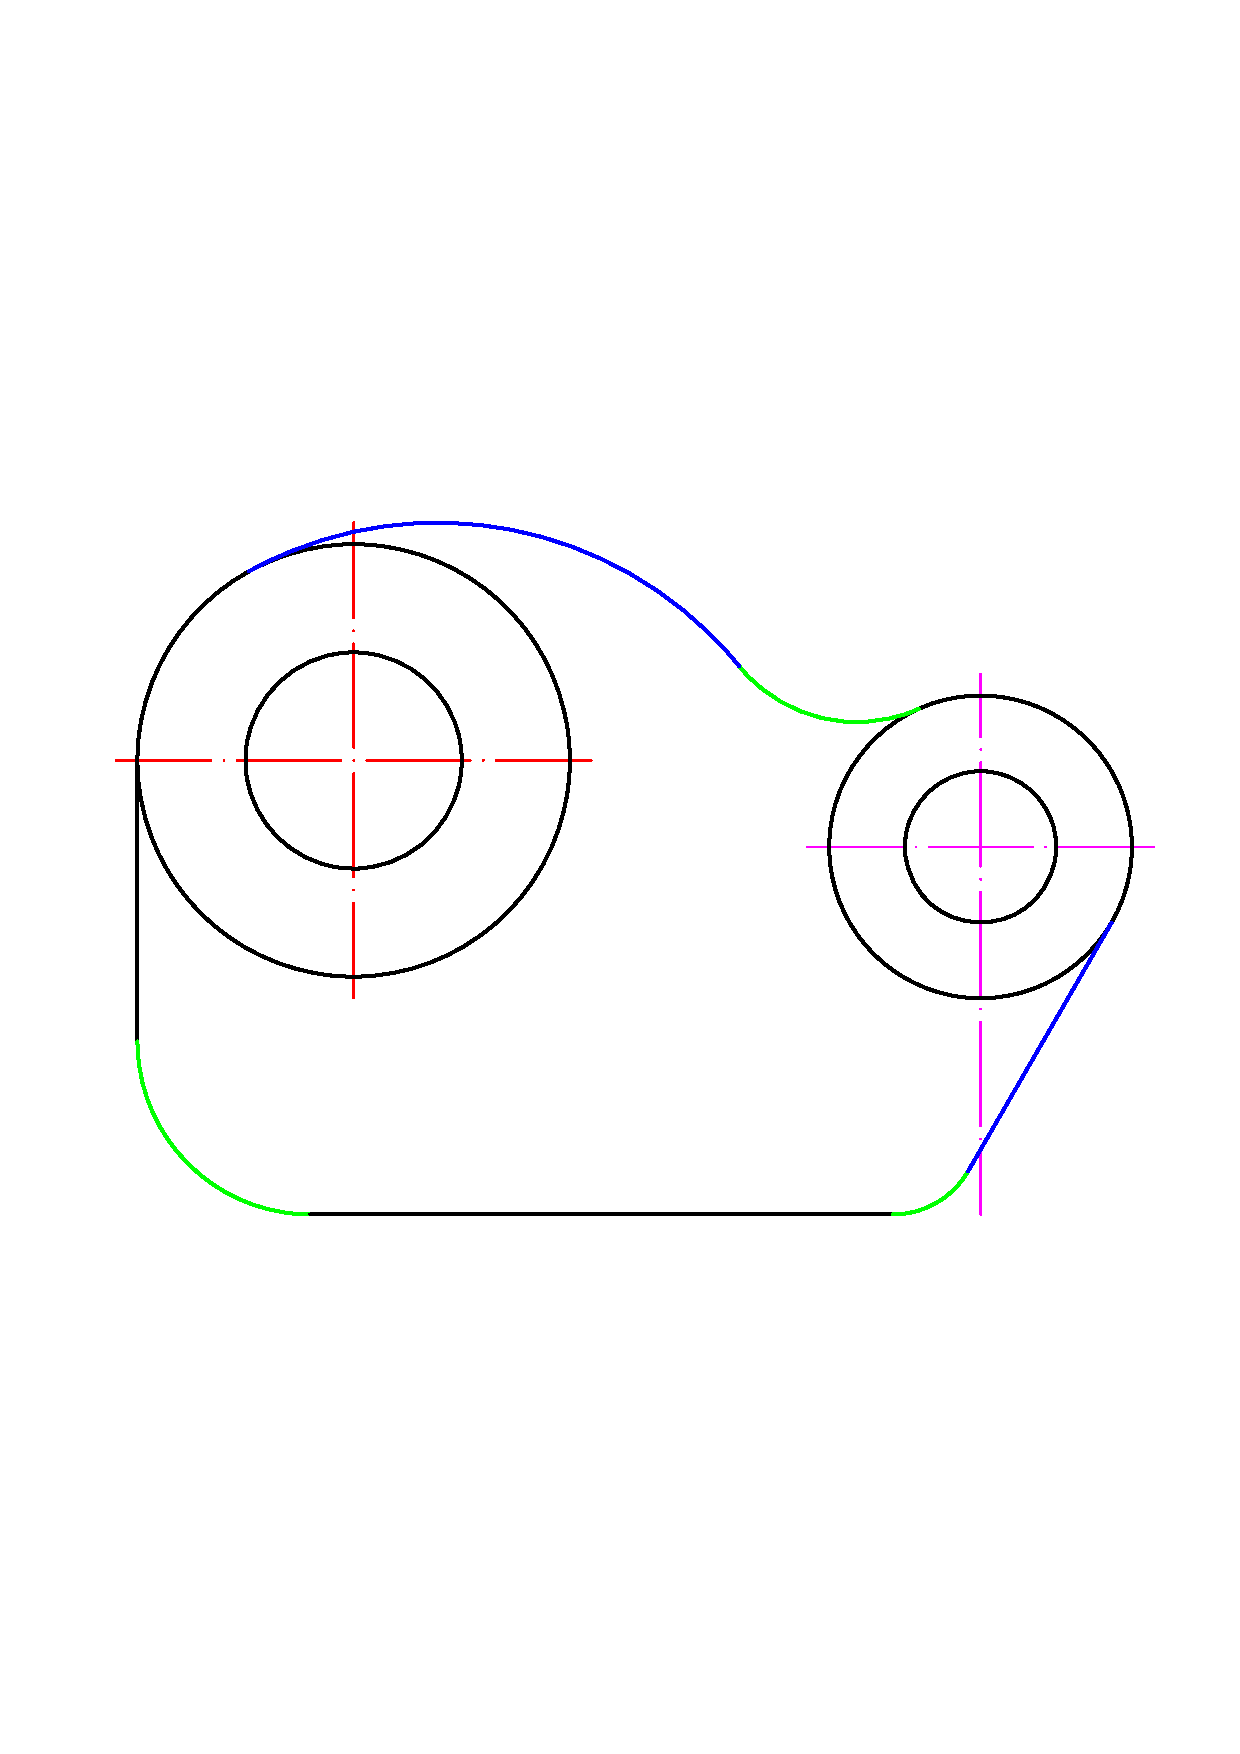
\includegraphics[scale=0.2]{biaozu4.pdf}}
\caption{平面图形中的线段分析}
\end{figure}

爸爸:垫片零件图(图\ref{fig:tiaoyafadianpian})中的图线性质是怎样的?

秦奋:垫片零件图中的图线都是已知线段。

爸爸:你分析得很到位,我们现可以开始零件的三维建模了。
\section{拉伸建模法}
\subsection{绘制垫片主视图}\label{sec:dianpian}
\begin{procedure}
\item 设置图层。

由于图\ref{fig:tiaoyafadianpian}中不仅有实线还有中心线。中心线是用于表达图元对称中心位置的图线。为便于对各类图线进行统一管理,我们需要进行图层设置。所谓图层就是将属性相同的对象绘制在一张类似于透明的纸上,将不同属性的对象绘制在不同的透明的纸上,以便实现图形对象的分类管理,最后将所有的透明的纸叠加在一起就构成了整个图形。设置【图层】的方法有:
\begin{itemize}
\item 键盘输入LAYER或LA。
\item 点击【格式】菜单中的【图层】项。
\item 点击【工具栏】中的【图层】图标
\includegraphics[scale=0.6]{layertool.png}。
\end{itemize}
以上三种方法都将启动图\ref{fig:layerdialog}所示的【图层特性管理器】对话框。
\begin{figure}[htbp]
\centering
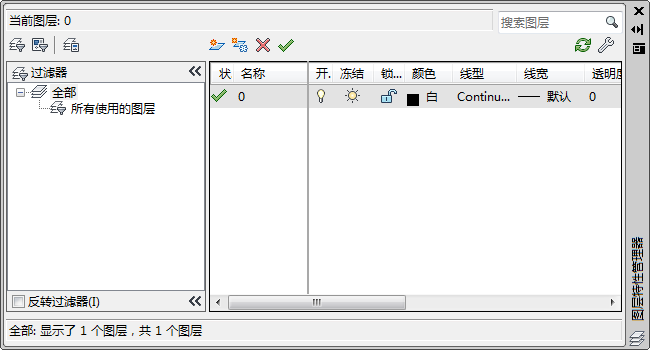
\includegraphics[scale=0.4]{layerdialog.png}
\caption{【图层特性管理器】对话框}\label{fig:layerdialog}
\end{figure}

单击【图层特性管理器】对话框中的【新建图层】图标
\includegraphics[scale=0.6]{newlayer.png},新建一个中心线图层和实线图层,分别取名为“中心线”和“实线”。

\begin{figure}[htbp]
\centering
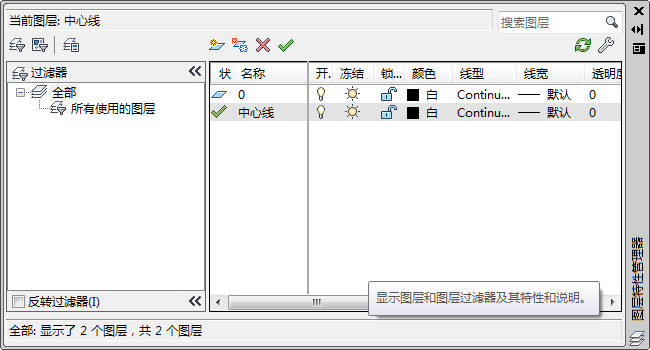
\includegraphics[scale=0.4]{layersetresult1.png}
\caption{新建图层结果}\label{fig:layersetresult1}
\end{figure}

选中新建的“中心线”图层,单击【置为当前】图标
\includegraphics[scale=0.6]{setcurrentlayer.png},将“中心线”图层置为当前,其结果如图\ref{fig:layersetresult1}所示。

为了区别各个图层的对象,通常需要设置各个图层的颜色。为此我们将实线图层的颜色设置为红色,将中心线图层设置为蓝色。具体设置方法是:单击“实线”图层
\includegraphics[scale=0.5]{solidlayerset.png}中的
\includegraphics[scale=0.6]{coloricon.png}图标将弹出如图\ref{fig:colorselect}所示的【选择颜色】对话框,选择红色颜色,并单击【确定】。“中心线”层的设置方法与“实线”层的设置方法相同。

\begin{figure}[htbp]
\centering
\begin{floatrow}
\ffigbox{\caption{【选择颜色】对话框}\label{fig:colorselect}}{
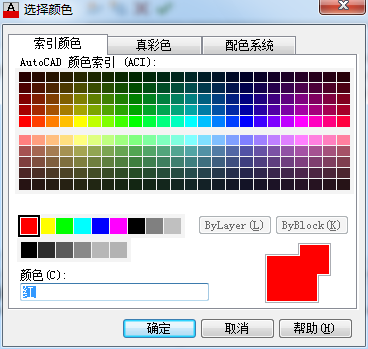
\includegraphics[scale=0.37]{colorselect.png}
}
\ffigbox{\caption{【线宽】对话框}\label{fig:linewidthselect}}{
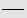
\includegraphics[scale=0.4]{linewidthselect.png}
}
\end{floatrow}
\end{figure}

接下来设置实线层的线宽,单击实线层中的线宽图标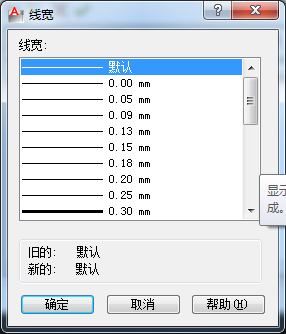
\includegraphics[scale=0.6]{linewidthset.png},弹出如图\ref{fig:linewidthselect}所示的【线宽】对话框,选择0.7mm的线宽作为实线层的线宽,单击确定。

接下来,按照规定将中心线图层的线型设置为CENTER图线。具体设置方法为:单击“中心线”层中的线型名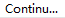
\includegraphics[scale=0.6]{linetypeicon.png}l图标,弹出如图\ref{fig:linetypeset}所示的【选择线型】对话框。此时还没我所需要的线型,需要单击对话框中的【加载...】按钮,弹出如图\ref{fig:loadlinetype}所示的【加载或重载线型】对话框,选择CENTER图线,并确定,以完成线型加载。最后在【选择线型】对话框中选中新加载的CENTER图线,再一次单击确定,完成线型的设置。
\begin{figure}[htbp]
\centering
\begin{floatrow}
\ffigbox{\caption{【选择线型】对话框}\label{fig:linetypeset}}{
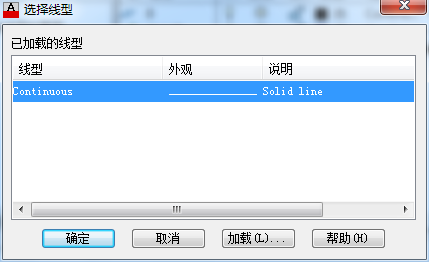
\includegraphics[scale=0.4]{linetypeset.png}
}
\ffigbox{\caption{【加载或重载线型】对话框}\label{fig:loadlinetype}}{
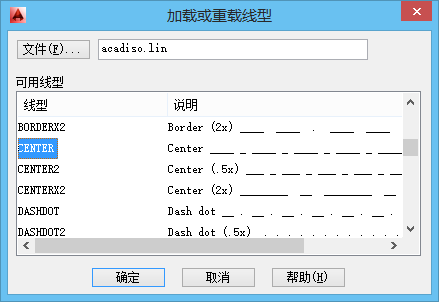
\includegraphics[scale=0.33]{loadlinetype.png}
}
\end{floatrow}
\end{figure}

通过上述操作就能够得到图\ref{fig:layersetresult2}所示图层设置结果。完成设置后单击对话框中的关闭按钮返加绘图界面。
\begin{figure}[htbp]
\centering
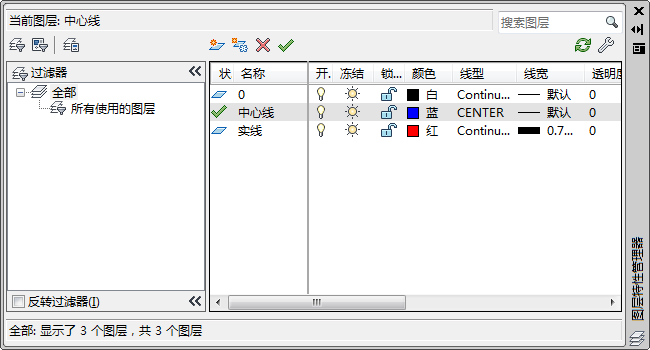
\includegraphics[scale=0.4]{layersetresult2.png}
\caption{图层设置结果}\label{fig:layersetresult2}
\end{figure}

\item 切换视图为主视图。【视图】菜单中【三维视图】子菜单中的【前视图】。
\item 绘制中心线,其结果如图\ref{fig:centerresult}所示。

用【构造线】命令绘制出对称中心线。【构造线】命令的启动方法有:
\begin{itemize}
\item 键盘输入XLINE或XL。
\item 点击【绘图】菜单中的【构造线】项。
\item 点击【绘图】工具栏中的【构造线】图标
\includegraphics[scale=0.6]{xlinetool.png}。
\end{itemize}
\begin{lstlisting}
|命令: XLINE|
|指定点或 [水平(H)/垂直(V)/角度(A)/二等分(B)/偏移(O)]: 52,52|
|指定通过点:$ @1<0$|
|指定通过点:$ @1<90$|
|指定通过点:|
\end{lstlisting}

用CIRCLE命令绘制$\diameter 84$的中心线圆。
\begin{lstlisting}
|命令: CIRCLE|
|指定圆的圆心或 [三点(3P)/两点(2P)/切点、切点、半径(T)]:INT|
|指定圆的半径或 [直径(D)]: 42|
\end{lstlisting}
\item 切换图层为“实线”层。切换图层的方法有:
\begin{itemize}
\item 在【工具栏】中点击
\includegraphics[scale=0.6]{layercontral.png}图标,从弹出的列表中选择“实线”项,即可完成图层的切换。
\item 用【图层特性管理器】将“实线”层设置为当前。
\end{itemize}
\item 绘制圆。

用对称中心线的交点作$\diameter 104$、$\diameter 53$和$\diameter 8$的圆,其结果如图\ref{fig:dianpiancircle}所示
首先绘制$\diameter 104$的圆。
\begin{lstlisting}
|命令: circle|
|指定圆的圆心或 [三点(3P)/两点(2P)/切点、切点、半径(T)]:int|
|指定圆的半径或 [直径(D)] $<42.0000>$: 52|
\end{lstlisting}
再绘制$\diameter 53$的圆。
\begin{lstlisting}
|命令: circle|
|指定圆的圆心或 [三点(3P)/两点(2P)/切点、切点、半径(T)]:|
|指定圆的半径或 [直径(D)]$ <52.0000>$: 26.5|
\end{lstlisting}
最后绘$\diameter 8$的圆。
\begin{lstlisting}
|命令: circle|
|指定圆的圆心或 [三点(3P)/两点(2P)/切点、切点、半径(T)]:|
|指定圆的半径或 [直径(D)] $<26.5000>$: 4|
\end{lstlisting}

\begin{figure}[htbp]
\centering
\subfloat[]{\label{fig:centerresult}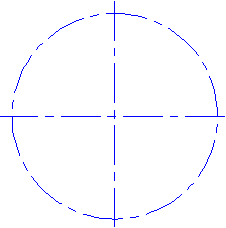
\includegraphics[scale=0.5]{centerresult.png}}\hspace{20pt}
\subfloat[]{\label{fig:dianpiancircle}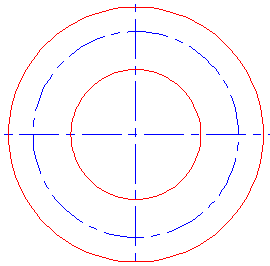
\includegraphics[scale=0.4]{dianpiancircle.png}}
\caption{绘制中心线和圆}
\end{figure}
\item 阵列圆。环形阵列的启动方法有:
\begin{itemize}
\item 键盘输入ARRAYPLOAY
\item 点击【修改】菜单中【阵列】子菜单中的【环形阵列】项
\item 点击【修改】工具栏中的【环形阵列】图标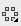
\includegraphics[scale=0.6]{arrayploaytool.png}。
\end{itemize}

\begin{figure}[htbp]
\centering
\subfloat[]{\label{fig:arraypolayselect}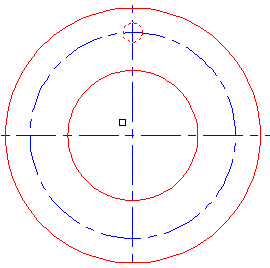
\includegraphics[scale=0.3]{arraypolayselect.png}}\hspace{20pt}
\subfloat[]{\label{fig:arraypolaycenter}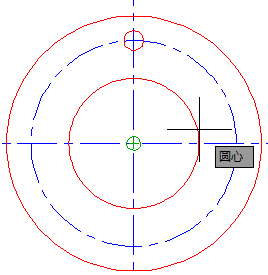
\includegraphics[scale=0.3]{arraypolaycenter.png}}\hspace{20pt}
\subfloat[]{\label{fig:arraypolayresult}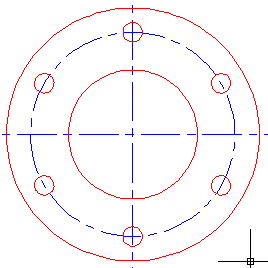
\includegraphics[scale=0.3]{arraypolayresult.png}}
\caption{环形阵列过程}
\end{figure}

启动阵列后要求选择需要阵列的对象,我们选择图\ref{fig:arraypolayselect}所示的$\diameter 8$的圆做为要阵列的对象,并结束对象选择。
\begin{lstlisting}
|命令: ARRAYPOLAR|
|选择对象: 找到 1 个|
|选择对象:|
|类型 = 极轴  关联 = 是|
\end{lstlisting}
接下来指定阵列中,以图\ref{fig:arraypolaycenter}所示的方式选择圆心作为阵列的中心点。
\begin{lstlisting}
|指定阵列的中心点或 [基点(B)/旋转轴(A)]:|
\end{lstlisting}
默认情况下将产生图\ref{fig:arraypolayresult}所示的由6个圆组成的环形阵列。若要产生其它数目的环形阵列,则需要使用【项目(i)】选项,并指定阵列数;若要产生非360度填充角度,则需要使用【直译角度(F)】选项,并指定填充角度。
\begin{lstlisting}
|选择夹点以编辑阵列或 [关联(AS)/基点(B)/项目(I)/项目间角度(A)/填|
|充角度(F)/行(ROW)/层(L)/旋转项目(ROT)/退出(X)] $<$退出$>$:|
\end{lstlisting}
\end{procedure}
\endinput
\subsection{拉伸构建垫片三维建模}
\begin{procedure}
\item关闭“中心线”层,关闭后的结果如图\ref{fig:offcenterlayer}所示。图层的关闭方法有:
\begin{itemize}
\item 单击【工具栏】中的
\includegraphics[scale=0.6]{layercontral.png}图标,从弹出列表中点击“中心线”层中的
\includegraphics[scale=0.6]{layeronoffset.png}图标,使其变为
\includegraphics[scale=0.6]{layeroffstatus.png}灰色状态。
\item 打开【图层特性管理器,点击“中心线”层中的
\includegraphics[scale=0.6]{layeronoffset.png}图标,使其变为
\includegraphics[scale=0.6]{layeroffstatus.png}灰色状态。
\end{itemize}
\item 通过拉伸操作构建圆柱体,拉伸结果如图\ref{fig:dianpianextrude}所示。
\begin{lstlisting}
|命令: EXTRUDE|
|当前线框密度:  ISOLINES=4,闭合轮廓创建模式 = 实体|
|选择要拉伸的对象或 [模式(MO)]: 指定对角点: 找到 8 个|
|选择要拉伸的对象或 [模式(MO)]:|
|指定拉伸的高度或 [方向(D)/路径(P)/倾斜角(T)/表达式(E)]: 2|
\end{lstlisting}
\item 切换视图为西南等轴测图。点击【视图】菜单中【三维视图】子菜单中的【西南等轴测】。
\item 进行差集操作,构建垫片的三维模型
\begin{lstlisting}
|命令: subtract |
|选择要从中减去的实体、曲面和面域...|
|选择对象: 找到 1 个|
|选择对象:  选择要减去的实体、曲面和面域...|
|选择对象: 找到 1 个|
|选择对象: 找到 1 个,总计 2 个|
|选择对象: 找到 1 个,总计 3 个|
|选择对象: 找到 1 个,总计 4 个|
|选择对象: 找到 1 个,总计 5 个|
|选择对象: 找到 1 个,总计 6 个|
|选择对象: 找到 1 个,总计 7 个|
|选择对象:|
\end{lstlisting}
\begin{figure}[htbp]
\centering
\subfloat[]{\label{fig:offcenterlayer}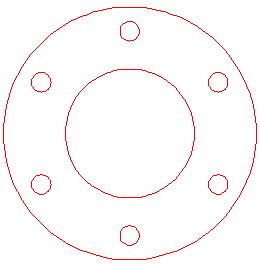
\includegraphics[scale=0.45]{offcenterlayer.png}}\hspace{20pt}
\subfloat[]{\label{fig:dianpianextrude}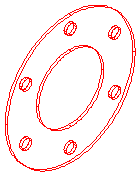
\includegraphics[scale=0.65]{dianpianextrude.png}}\hspace{20pt}
\subfloat[]{\label{fig:dianpiansolid}
\includegraphics[scale=0.65]{dianpiansolid.png}}
\caption{垫片拉伸建模过程}
\end{figure}
\item 设置视觉样式为真实,其结果如图\ref{fig:dianpiansolid}所示。
\item 将垫片模型保存为“调压阀垫片立体图.dwg”。
\end{procedure}

\section{旋转建模法}
\subsection{绘制垫片特征图}
\begin{procedure}
\item 设置图层。

新建“中心线”和“实线”两个图层,具体设计请参看\ref{sec:dianpian}节的图层设置相关内容。
\item  切换视图为主视图。
\item 绘制中心线。

中心线绘制结果如图\ref{fig:dianpiancenterline1}所示。
绘制对称中心线。
\begin{lstlisting}
|命令: xline|
|指定点或 [水平(H)/垂直(V)/角度(A)/二等分(B)/偏移(O)]:|
|指定通过点:$@1<0$|
|指定通过点:$@1<90$|
|指定通过:|
\end{lstlisting}
通过偏移的方法产生$\phi 8$圆孔的中心线。
\begin{lstlisting}
|命令:OFFSET|
|当前设置: 删除源=否  图层=源  OFFSETGAPTYPE=0|
|指定偏移距离或 [通过(T)/删除(E)/图层(L)] $<$通过$>$:  42|
|选择要偏移的对象,或 [退出(E)/放弃(U)] $<$退出$>$:|
|指定要偏移的那一侧上的点,或 [退出(E)/多个(M)/放弃(U)] $<$退出$>$:|
|选择要偏移的对象,或 [退出(E)/放弃(U)] $<$退出$>$:
\end{lstlisting}
\item 将图层切换为实线层
\begin{figure}[htbp]
\centering
\subfloat[]{\label{fig:dianpiancenterline1}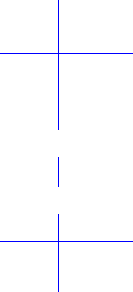
\includegraphics[scale=0.6]{dianpiancenterline1.png}}\hspace{40pt}
\subfloat[]{\label{fig:dianpianleft1}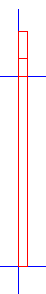
\includegraphics[scale=0.6]{dianpianleft1.png}}
\caption{垫片特征图绘制}
\end{figure}
\item 绘用于旋转操作的关键特征。

使用【矩形】命令绘制左视图中的关键特征,其结果如图\ref{fig:dianpianleft1}所示。绘制用于旋转产生$\phi 104$直径圆柱的特征矩形。
\begin{lstlisting}
|命令: rectang|
|指定第一个角点或 [倒角(C)/标高(E)/圆角(F)/厚度(T)/宽度(W)]:|
|指定另一个角点或 [面积(A)/尺寸(D)/旋转(R)]: @2,52|
\end{lstlisting}
绘制用于旋转生成$\phi 8$直径圆柱的特征矩形。
\begin{lstlisting}
|命令: rectang|
|指定第一个角点或 [倒角(C)/标高(E)/圆角(F)/厚度(T)/宽度(W)]:|
|指定另一个角点或 [面积(A)/尺寸(D)/旋转(R)]: @2,4|
\end{lstlisting}
绘制用于旋转生成$\phi 53$直径圆柱的特征矩形。
\begin{lstlisting}
|命令: rectang|
|指定第一个角点或 [倒角(C)/标高(E)/圆角(F)/厚度(T)/宽度(W)]:|
|指定另一个角点或 [面积(A)/尺寸(D)/旋转(R)]: @2,26.5|
\end{lstlisting}
\end{procedure}

\endinput
\subsection{旋转构建垫片的三维模型}
\begin{procedure}
\item 通过建模中的【旋转】操作产生三个圆柱。

旋转产生$\phi 104$直径圆柱。
\begin{lstlisting}
|命令: REVOLVE|
|当前线框密度:  ISOLINES=4,闭合轮廓创建模式 = 实体|
|选择要旋转的对象或 [模式(MO)]: 找到 1 个|
|选择要旋转的对象或 [模式(MO)]:|
|指定轴起点或根据以下选项之一定义轴 [对象(O)/X/Y/Z] $<$对象$>$:|
|指定轴端点:|
|指定旋转角度或 [起点角度(ST)/反转(R)/表达式(EX)] $<360>$:|
\end{lstlisting}
旋转产生$\phi 53$直径圆柱
\begin{lstlisting}
|命令:  REVOLVE|
|当前线框密度:  ISOLINES=4,闭合轮廓创建模式 = 实体|
|选择要旋转的对象或 [模式(MO)]: 找到 1 个|
|选择要旋转的对象或 [模式(MO)]:|
|指定轴起点或根据以下选项之一定义轴 [对象(O)/X/Y/Z] $<$对象$>$:|
|指定轴端点:|
|指定旋转角度或 [起点角度(ST)/反转(R)/表达式(EX)]$ <360>$:|
\end{lstlisting}
旋转产生$\phi 8$直径圆柱
\begin{lstlisting}
|命令:  REVOLVE|
|当前线框密度:  ISOLINES=4,闭合轮廓创建模式 = 实体|
|选择要旋转的对象或 [模式(MO)]: 找到 1 个|
|选择要旋转的对象或 [模式(MO)]:|
|指定轴起点或根据以下选项之一定义轴 [对象(O)/X/Y/Z] $<$对象$>$:|
|指定轴端点:|
|指定旋转角度或 [起点角度(ST)/反转(R)/表达式(EX)]$ <360>$:|
\end{lstlisting}
\item 关闭“中心线”图层。
\item 切换视图为西南等轴测图。

切换后的结果如图\ref{fig:3darray}所示。
\begin{figure}[htbp]
\centering
\subfloat[]{\label{fig:3darray}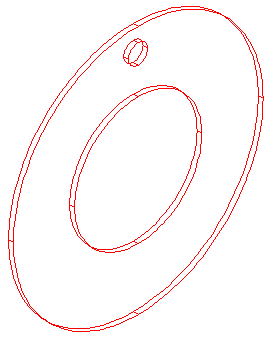
\includegraphics[scale=0.5]{3darray.png}}\hspace{30pt}
\subfloat[]{\label{fig:3darrayselect}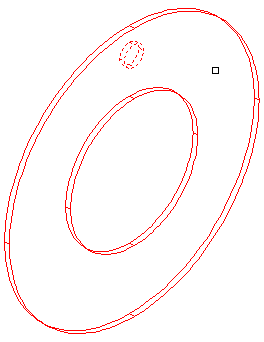
\includegraphics[scale=0.5]{3darrayselect.png}}\hspace{30pt}
\subfloat[]{\label{fig:3darrayresult}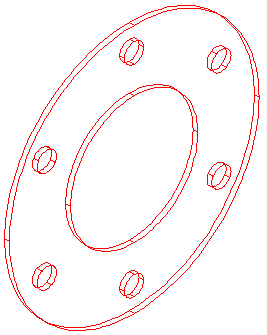
\includegraphics[scale=0.5]{3darrayresult.png}}
\caption{三维阵列过程}
\end{figure}
\item 阵列产生圆柱体。

用【三维阵列】命令阵列$\diameter 8$的圆柱,其结果如图\ref{fig:3darrayresult}所示。

启动【三维阵列】命令的方法有:
\begin{itemize}
\item 键盘输入3DARRAY\index{3darray}。
\item 【修改】$\rightarrow$【三维操作】$\rightarrow$【三维阵列】。
\item 【建模】$\triangleright$【三维阵列】图标
\includegraphics[scale=0.6]{3darraytool.png}。
\end{itemize}

按图\ref{fig:3darrayselect}所示的选择$\diameter 8$圆柱作为三维阵列对象
\begin{lstlisting}
|命令: 3darray|
|选择对象: 找到 1 个|
|选择对象:|
\end{lstlisting}
指定三维阵列的类型为环形。
\begin{lstlisting}
|输入阵列类型 [矩形(R)/环形(P)]$<$矩形$>$:p|
\end{lstlisting}
指定三维阵列项目的数量为6个。
\begin{lstlisting}
|输入阵列中的项目数目: 6|
\end{lstlisting}
指定三维阵列项目的填充角度为360度。
\begin{lstlisting}
|指定要填充的角度 (+=逆时针, -=顺时针)$ <360>$:|
\end{lstlisting}
指定是否旋转阵列对象。
\begin{lstlisting}
|旋转阵列对象? [是(Y)/否(N)] $<Y>$:|
\end{lstlisting}
选择$\diameter 104$圆柱的后底圆圆心为阵列中心线第一端点。
\begin{lstlisting}
|指定阵列的中心点:|
\end{lstlisting}
选择$\diameter 104$圆柱的前顶圆圆心为阵列中心线第二端点。
\begin{lstlisting}
|指定旋转轴上的第二点:|
\end{lstlisting}
\item 用差集操作完成垫片的三维建模操作。
\begin{lstlisting}
|命令: subtract |
|选择要从中减去的实体、曲面和面域...|
|选择对象: 找到 1 个|
|选择对象:  选择要减去的实体、曲面和面域...|
|选择对象: 找到 1 个|
|选择对象: 找到 1 个,总计 2 个|
|选择对象: 找到 1 个,总计 3 个|
|选择对象: 找到 1 个,总计 4 个|
|选择对象: 找到 1 个,总计 5 个|
|选择对象: 找到 1 个,总计 6 个|
|选择对象: 找到 1 个,总计 7 个|
|选择对象:|
\end{lstlisting}
\item 设置视觉样式为真实,其结果如图\ref{fig:dianpiansolid}所示。设置方法为:点击【视图】菜单中【视觉样式】子菜单中的【真实】项。
\item 将垫片模型保存为“调压阀垫片立体图.dwg”。
\end{procedure}
\endinput
\section{实体建模法}
\begin{procedure}
\item 设置图层。

新建“中心线”和“实线”两个图层,具体设计请参看\ref{sec:dianpian}节的图层设置相关内容。
\item 切换视图为主视图。

\item 绘制中心线,用以辅助绘图。

绘制对称中心线。
\begin{lstlisting}
|命令: XLINE|
|指定点或 [水平(H)/垂直(V)/角度(A)/二等分(B)/偏移(O)]: 52,52|
|指定通过点:$ @1<0$|
|指定通过点:$ @1<90$|
|指定通过点:|
\end{lstlisting}
绘制$\phi 84$中心线圆,其结果如图\ref{fig:dianpiancenterline}所示。
\begin{lstlisting}
|命令: circle|
|指定圆的圆心或 [三点(3P)/两点(2P)/切点、切点、半径(T)]:|
|指定圆的半径或 [直径(D)]: 42|
\end{lstlisting}
\begin{figure}[htbp]
\centering
\begin{floatrow}
\ffigbox{\caption{绘中心线}\label{fig:dianpiancenterline}}{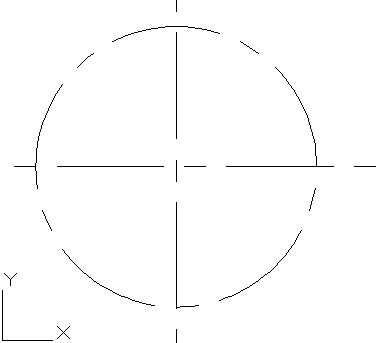
\includegraphics[scale=0.35]{dianpiancenterline.png}}
\ffigbox{\caption{绘$\phi 108$圆柱体}\label{fig:dianpian1}}{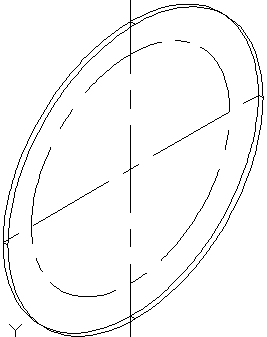
\includegraphics[scale=0.35]{dianpian1.png}}
\end{floatrow}
\end{figure}
\item 切换视图为西南等轴测图。

点击【视图】菜单中【三维视图】子菜单中的【西南等轴测】。
\item 用【圆柱体】命令绘制圆柱体。

【圆柱体】命令的启动方法有:
\begin{itemize}
\item 键盘输入CYLINDER\index{cylinder}或CYL。
\item 【绘图】$\rightarrow$【建模】$\rightarrow$【圆柱体】。
\item 【建模】$\triangleright$【圆柱体】图标
\includegraphics[scale=0.6]{cylinder.png}。
\end{itemize}
绘制$\phi 108$直径的圆柱体,其结果如图\ref{fig:dianpian1}所示。
\begin{lstlisting}
|命令: cylinder|
|指定底面的中心点或 [三点(3P)/两点(2P)/切点、切点、半径(T)/椭|
|圆(E)]:int|
|指定底面半径或 [直径(D)]: 54|
|指定高度或 [两点(2P)/轴端点(A)]$ <2.0000>$: 2|
\end{lstlisting}
绘制$\phi 53$直径的圆柱体,其结果如图\ref{fig:dianpian2}所示。
\begin{lstlisting}
|命令: cylinder|
|指定底面的中心点或 [三点(3P)/两点(2P)/切点、切点、半径(T)/椭|
|圆(E)]:int|
|指定底面半径或 [直径(D)]$ <54.0000>$: 26.5|
|指定高度或 [两点(2P)/轴端点(A)] $<2.0000>$:|
\end{lstlisting}
绘制$\phi 8$直径的圆柱体,其结果如图\ref{fig:dianpian3}所示。
\begin{lstlisting}
|命令: cylinder|
|指定底面的中心点或 [三点(3P)/两点(2P)/切点、切点、半径(T)/椭|
|圆(E)]:int|
|指定底面半径或 [直径(D)] $<26.5000>$: 4|
|指定高度或 [两点(2P)/轴端点(A)]$ <2.0000>$:|
\end{lstlisting}
\begin{figure}[htbp]
\centering
\begin{floatrow}
\ffigbox{\caption{绘$\phi 53$圆柱体}\label{fig:dianpian2}}{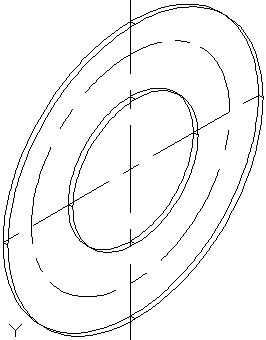
\includegraphics[scale=0.5]{dianpian2.png}}\hspace{30pt}
\ffigbox{\caption{绘$\phi 8$圆柱体}\label{fig:dianpian3}}{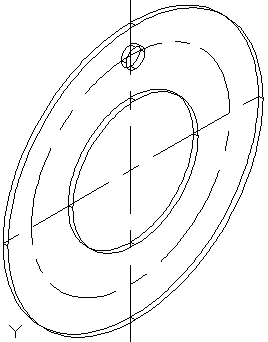
\includegraphics[scale=0.5]{dianpian3.png}}
\end{floatrow}
\end{figure}
\item 关闭“中心线”图层。
\item 三维阵列$\diameter 8$的圆柱,其结果如图\ref{fig:dianpian4}所示。
\newpage
\begin{lstlisting}
|命令: 3darray|
|选择对象: 找到 1 个|
|选择对象:|
|输入阵列类型 [矩形(R)/环形(P)]$<$矩形$>$:p|
|输入阵列中的项目数目: 6|
|指定要填充的角度 (+=逆时针, -=顺时针)$ <360>$:|
|旋转阵列对象? [是(Y)/否(N)] $<Y>$:|
|指定阵列的中心点:|
|指定旋转轴上的第二点:|
\end{lstlisting}
\item 用差集操作完成垫片的三维建模操作。
\begin{lstlisting}
|命令: subtract |
|选择要从中减去的实体、曲面和面域...|
|选择对象: 找到 1 个|
|选择对象:  选择要减去的实体、曲面和面域...|
|选择对象: 找到 1 个|
|选择对象: 找到 1 个,总计 2 个|
|选择对象: 找到 1 个,总计 3 个|
|选择对象: 找到 1 个,总计 4 个|
|选择对象: 找到 1 个,总计 5 个|
|选择对象: 找到 1 个,总计 6 个|
|选择对象: 找到 1 个,总计 7 个|
|选择对象:|
\end{lstlisting}
\begin{figure}[htbp]
\centering
\begin{floatrow}
\ffigbox{\caption{阵列$\phi 8$圆柱体}\label{fig:dianpian4}}{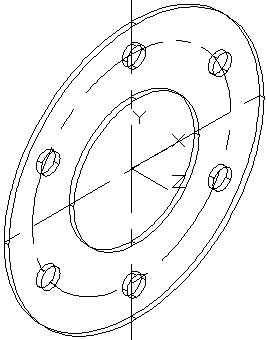
\includegraphics[scale=0.5]{dianpian4.png}}\hspace{30pt}
\ffigbox{\caption{垫片三维模型}\label{fig:dianpian5}}{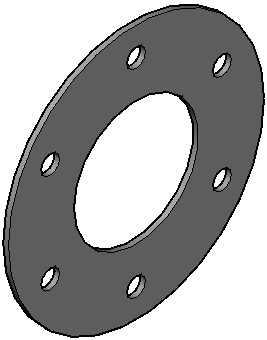
\includegraphics[scale=0.5]{dianpian5.png}}
\end{floatrow}
\end{figure}
\item 设置视觉样式为真实,其结果如图\ref{fig:dianpian5}所示。设置方法为:点击【视图】菜单中【视觉样式】子菜单中的【灰度】项。
\item 将垫片模型保存为“调压阀垫片立体图.dwg”。
\end{procedure}

\endinput
%%%%%%%%%%%%%%教案头%%%%%%%%%%%%%%%%%%%%%%%%%%%%%%%
\mode<article>{

\begin{longtable}{|m{20mm}|m{20mm}|m{20mm}|m{20mm}|m{20mm}|m{28mm}|}
\caption*{\huge 教案头}\\
\hline
\endfirsthead
\multicolumn{6}{l}{(续表)}\\
\hline
\endhead
\hline
\multicolumn{6}{l}{\itshape 接下一页表格.......}\\ [2ex]
\endfoot
\hline
\endlastfoot
\centering{授课单元}&\multicolumn{3}{m{60mm}|}{\centering 2.5传递函数和信号流图}&\centering{授课日期}&2014年03月13日 \\
\hline
\centering 授课地点 & \multicolumn{3}{m{60mm}|}{B6-204}&\centering 授课学时 & 2 \\
\hline
& \multicolumn{2}{m{40mm}|}{能力目标} & \multicolumn{2}{m{40mm}|}{知识目标}&素质目标 \\
\cline{2-6}
\centering 教学目标&\multicolumn{2}{m{40mm}|}{\begin{enumerate}
\item 能够将方框图转化为信号流图
\item 能够应用梅逊增益公式求解系统的传递函数
\end{enumerate} }&\multicolumn{2}{m{40mm}|}{\begin{enumerate}
\item 掌握信号流图的画法
\item 掌握梅逊增益公式
\end{enumerate}} & {\qquad}\\
\hline
\centering 能力训练任务或案例 &\multicolumn{5}{m{108mm}|}{ }\\
\hline
\centering 教学重点 & \multicolumn{5}{m{108mm}|}{\begin{enumerate}
\item 梅逊增益公式
\end{enumerate}}\\
\hline
\centering 教学难点与解决办法 &\multicolumn{5}{m{108mm}|}{\begin{enumerate}
\item 难点:梅逊增益公式
\item 解决方法:用实例进行分析讲解
\end{enumerate}}\\
\hline
\centering 德育内容 &\multicolumn{5}{m{108mm}|}{无}\\
\hline
 &教材 & \multicolumn{4}{m{88mm}|}{计算机控制原理与应用}\\
\cline{2-6}& 教学资源 &\multicolumn{4}{m{88mm}|}{PPT}\\
\cline{2-6}\centering 使用的教学材料& 主要教学仪器设备和工具等 &\multicolumn{4}{m{88mm}|}{投影机、MATLAB}\\
\cline{2-6}& 主要耗材 &\multicolumn{4}{m{88mm}|}{无}\\
\hline
\centering 教学模式 &\multicolumn{2}{m{40mm}|}{知识讲授}&\centering 教学手段 &\multicolumn{2}{m{48mm}|}{多媒体教学}\\
\hline
\centering 学生成果与过程考核方式 &\multicolumn{5}{m{108mm}|}{无}
\end{longtable}
\clearpage

%%%%%%%%%%%%%%%教学实施过程%%%%%%%%%%%%%%%%%%%%%%%%%%%%
\begin{landscape}

\begin{longtable}{|m{10mm}|m{50mm}|m{50mm}|m{50mm}|m{15mm}|}
\caption*{\huge 教学组织与实施}\\
\hline
\endfirsthead
\multicolumn{5}{l}{\small 接上页}\\
\hline
\multicolumn{1}{|c|}{步骤}&\multicolumn{1}{c|}{教学内容}&\multicolumn{1}{c|}{教师活动}&\multicolumn{1}{c|}{学生活动}&\multicolumn{1}{c|}{时间}\\
\hline
\endhead

\multicolumn{5}{r}{\small 接下页}\\
\endfoot
\hline
\endlastfoot
\multicolumn{1}{|c|}{步骤}&\multicolumn{1}{c|}{教学内容}&\multicolumn{1}{c|}{教师活动}&\multicolumn{1}{c|}{学生活动}&\multicolumn{1}{c|}{时间}\\\hline
引入&\begin{enumerate}
\item 复习方框图的简化
\end{enumerate} &\begin{enumerate}
\item 通过提问了解学生对方框图的简化掌握情况
\end{enumerate} &\begin{enumerate}
\item 学生回简问题
\end{enumerate} &10 \\\hline
讲解&\begin{enumerate}
\item 信息号流图的定义和绘制方法
\end{enumerate}
 &\begin{enumerate}
\item 通过实例讲解信号流图的定义和绘制
\end{enumerate} &\begin{enumerate}
\item 学生倾听并记录
\end{enumerate} &15 \\\hline
练习&\begin{enumerate}
\item 将方框图转换为信号流图
\end{enumerate}
&\begin{enumerate}
\item 指定需要转换的方框图
\item 指导学生进行信号流图的绘制
\item 讲解正确结果
\end{enumerate} &\begin{enumerate}
\item 学生尝试将方框图转为信号流图
\item 学生展示绘制结果
\item 学生进行记录
\end{enumerate} &20 \\\hline
讲解&\begin{enumerate}
\item 用梅逊增益求解系统的传递函数
\end{enumerate}
 &\begin{enumerate}
\item 讲解梅逊增益公式
\item 讲解用梅逊增益公式求解系统传递函数的实例
\end{enumerate} &\begin{enumerate}
\item 学生记录笔记
\end{enumerate} &20 \\\hline
练习&
\begin{enumerate}
\item 用梅逊增益公式求解系统传递函数
\end{enumerate}
 &\begin{enumerate}
\item 指导学生进行系统传递函数求解
\item 讲解要点
\end{enumerate} &\begin{enumerate}
\item 学生尝试用梅逊公式求解系统传递函数
\item 学生记录笔记
\end{enumerate} &20 \\\hline
\centering 本次课总结(评价)&总结本课程内容 &进行知识总结 &学生倾听 &5 \\\hline
\centering 学生学习笔记或工单等检查情况&\multicolumn{4}{m{165mm}|}{\quad}\\\hline
\centering 课后作业&\multicolumn{4}{m{165mm}|}{2-19,2-20,2-21}\\\hline
\centering 教学体会&\multicolumn{4}{m{165mm}|}{\quad}\\
\end{longtable}

\end{landscape}
\clearpage
%%%%%%%%%%%%%%%%%%%%板书设计%%%%%%%%%%%%%%%%%%%%%%%%%%
\lecture{传递函数与信号流图}{chuandihanshu}
\begin{center}
{\huge 板书设计}
\end{center}
}
\mode<presentation>{ \section{传递函数与信号流图}
 \subsection{信号流图的定义}}
 \begin{frame}
 \uncover<+->{\begin{block}{信息流图的组成}
 \begin{itemize}
 \item<+-> 节点:表示变量或信号
 \item<+-> 支路:连接两个接点的有向线段
 \end{itemize}
 \end{block}}
 \uncover<+->{\begin{block}{信号流图的特点}
 \begin{itemize}
 \item<+-> 是系统代数方程的图形表示
 \item<+-> 不是唯一的
 \item<+-> 便于用梅逊增益公式求解系统传递函数
 \end{itemize}
 \end{block}}
 \end{frame}
 \begin{frame}
 \begin{block}{简化的特点}
 \begin{itemize}
 \item 传递函数具有唯一性
 \item 方框图不唯一
 \end{itemize}
 \end{block}
 \end{frame}
 \begin{frame}{用MatLab进行方框图化简}
 \begin{block}{串联}
 sys1=tf(num1,den1)
 
 sys2=tf(num2,den2)
 
 sys=series(sys1,sys2)
 \end{block}
 \begin{block}{并联}
 sys1=tf(num1,den1)
 
 sys2=tf(num2,den2)
 
 sys=parallel(sys1,sys2)
 \end{block}
 \end{frame}
 \begin{frame}
 \begin{block}{反馈连接}
sysg=[numg,deng]

sysh=[numh,denh]

sys=feedback(sysg,sysh)
 \end{block}
 \end{frame}

\endinput